\documentclass[11pt,a4paper]{article}

\usepackage[utf8]{inputenc}
\usepackage[T1]{fontenc}
\usepackage[french]{babel}
\usepackage{geometry}
\usepackage{graphicx}
\usepackage{hyperref}
\usepackage{xcolor}
\usepackage{array}
\usepackage{booktabs}
\usepackage{longtable}
\usepackage{enumitem}
\usepackage{float}

\geometry{margin=2.4cm}
\hypersetup{
  colorlinks=true,
  linkcolor=blue!45!black,
  urlcolor=blue!45!black
}
\setlist[itemize]{noitemsep, topsep=0.25em}
\setlist[enumerate]{noitemsep, topsep=0.25em}
\graphicspath{
  {../code/app mobile/UML/}
  {../code/boite hp/UML/}
  {../code/bracelet/UML/}
}

\title{\textbf{Starter}\\Rapport d'architecture et de compréhension du code}
\author{Projet personnel de réveil actif}
\date{\today}

\begin{document}

\maketitle
\tableofcontents
\newpage

\section{Objectif du projet}

Starter est un système de réveil personnel conçu pour rendre le retour au sommeil difficile. Le principe produit est volontairement simple: l'utilisateur prépare le réveil le soir, puis le système impose une activité physique minimale pendant les quinze premières minutes après l'heure configurée.

Le projet v1 est composé de trois parties actives:

\begin{itemize}
  \item une station de chevet, située dans \texttt{code/boite hp}, qui joue le rôle d'autorité centrale de l'alarme;
  \item un bracelet dédié, situé dans \texttt{code/bracelet}, qui mesure l'activité et la transmet à la station;
  \item une PWA mobile Vue/Vite, située dans \texttt{code/app mobile}, qui configure l'alarme et la musique via Supabase.
\end{itemize}

La règle centrale est que la station décide quand l'alarme démarre, quand le son est audible, et quand le cycle est terminé. La PWA ne déclenche pas l'alarme directement. Le bracelet ne stoppe pas l'alarme: il fournit uniquement une mesure d'activité que la station interprète.

\section{Vue d'ensemble de l'architecture}

Le flux de configuration v1 est:

\begin{center}
\texttt{PWA -> Supabase -> station}
\end{center}

Le flux d'activité est:

\begin{center}
\texttt{bracelet -> ESP-NOW -> station}
\end{center}

Supabase est utilisé pour stocker la musique, la sélection audio, la prochaine alarme et les états visibles par l'application. ESP-NOW est utilisé entre le bracelet et la station afin d'éviter un comportement WiFi lourd côté bracelet. Le transport ESP-NOW reste une hypothèse à valider physiquement sur la distance réelle d'utilisation.

\subsection{Règles produit non négociables}

\begin{itemize}
  \item La station reste l'autorité centrale.
  \item Supabase est utilisé pour la configuration et les musiques en v1.
  \item Le bracelet communique avec la station par ESP-NOW en v1.
  \item Il n'existe pas de bouton normal stop ou snooze.
  \item Le son est contrôlé par l'activité du bracelet pendant une fenêtre fixe de quinze minutes.
  \item Une panne technique bloquante doit placer le système dans un état de défaut visible.
  \item Un échec de streaming Supabase ne doit pas annuler le réveil: la station utilise un son local de secours.
\end{itemize}

\section{PWA mobile}

La PWA est l'interface utilisateur. Elle permet d'ajouter de la musique, de sélectionner une piste ou le fallback local, de configurer une alarme et de consulter l'état de la station et du bracelet.

\begin{center}
  \centering
  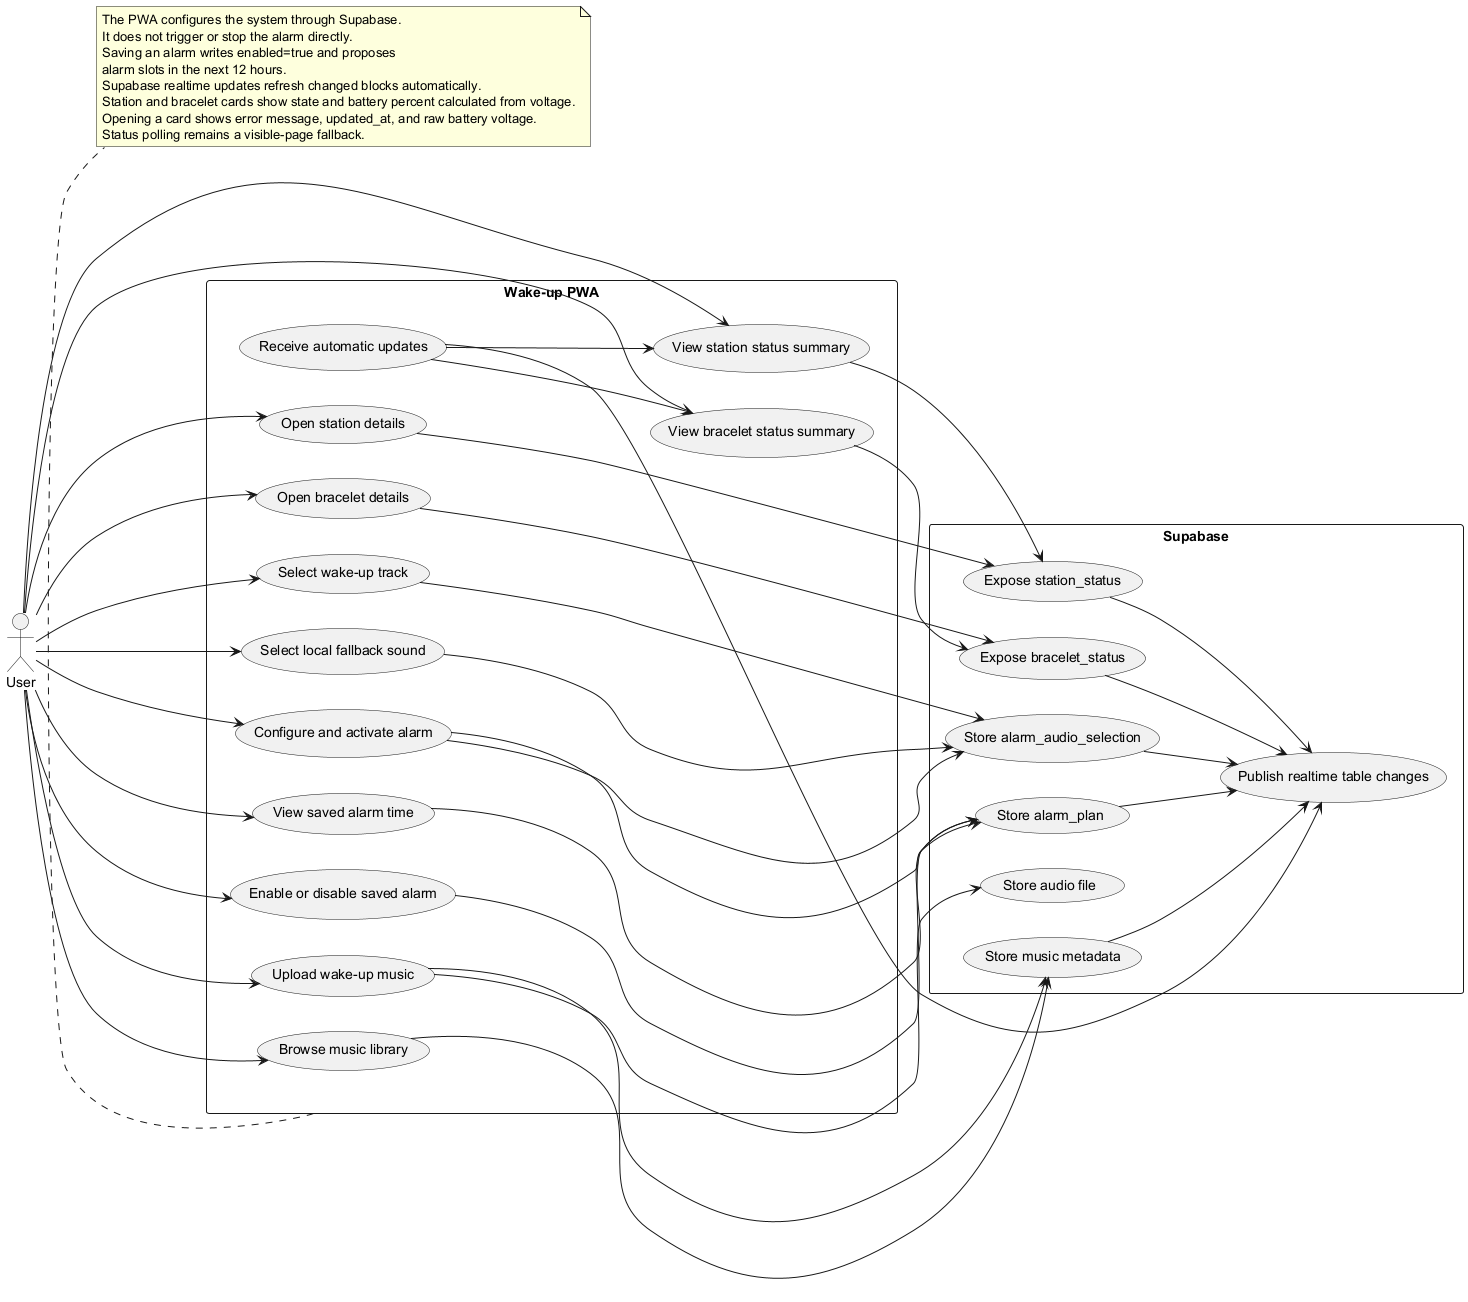
\includegraphics[width=\linewidth,height=0.72\textheight,keepaspectratio]{use_cases.png}
  \textbf{Diagramme: cas d'utilisation de la PWA}
\end{center}

\subsection{Responsabilités}

\begin{itemize}
  \item Uploader des fichiers audio vers le bucket Supabase \texttt{wake-up-music}.
  \item Créer les métadonnées dans \texttt{music\_tracks}.
  \item Écrire la configuration dans \texttt{alarm\_plan}.
  \item Écrire la sélection audio dans \texttt{alarm\_audio\_selection}.
  \item Lire \texttt{station\_status} et \texttt{bracelet\_status}.
  \item Afficher les défauts sans devenir l'autorité d'alarme.
\end{itemize}

Le code actuel utilise Vue 3, Vite, TypeScript, \texttt{@supabase/supabase-js} et \texttt{lucide-vue-next}. La configuration Supabase côté PWA passe par \texttt{VITE\_SUPABASE\_URL} et \texttt{VITE\_SUPABASE\_ANON\_KEY}. Cette clé anon est acceptable pour le prototype personnel, mais ce n'est pas un modèle de sécurité production.

\subsection{Fenêtre de sélection d'alarme}

La PWA propose des créneaux dans les douze prochaines heures, par pas de cinq minutes. Lorsqu'une alarme est sauvegardée, l'application incrémente la révision afin que la station puisse détecter une nouvelle configuration.

\section{Backend Supabase}

Supabase est le backend v1 pour les fichiers audio, la configuration de l'alarme et la publication des états. Le schéma SQL concret se trouve dans \texttt{database/supabase/v1\_schema.sql}.

\begin{longtable}{>{\ttfamily}p{0.28\linewidth}p{0.64\linewidth}}
\toprule
\normalfont Table & Rôle \\
\midrule
\endhead
music\_tracks & Bibliothèque des fichiers audio uploadés, avec titre, chemin de stockage, URL publique et disponibilité. \\
alarm\_plan & Ligne unique \texttt{main} contenant activation, date, heure locale, timezone et révision. \\
alarm\_audio\_selection & Ligne unique \texttt{main} contenant la source audio, la piste sélectionnée et le volume. \\
station\_status & État publié par la station: état courant, défaut, message, révision active, tension batterie. \\
bracelet\_status & État du bracelet vu par la station: état, défaut, message, tension batterie, dernière réception. \\
\bottomrule
\end{longtable}

Le bucket Supabase \texttt{wake-up-music} accepte les fichiers audio MPEG, WAV, OGG et MP4 audio jusqu'à 50 MiB. Les politiques RLS actuelles autorisent le client anon à lire et écrire les tables v1 et le bucket. Cette décision est explicitement limitée au prototype personnel.

\section{Station de chevet}

La station est un firmware PlatformIO Arduino pour ESP32. Elle synchronise l'heure, charge la configuration depuis Supabase, reçoit la télémétrie du bracelet, joue la musique sélectionnée et applique la logique d'alarme.

\begin{center}
  \centering
  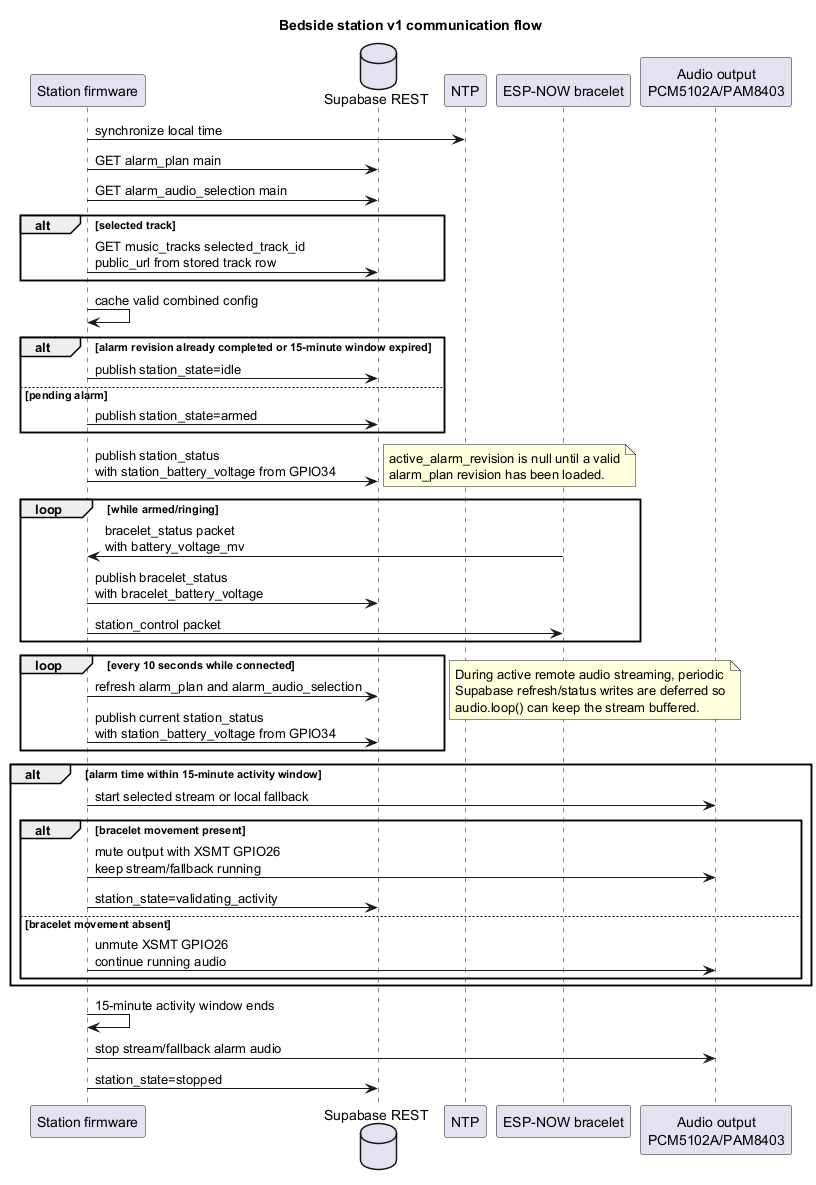
\includegraphics[width=\linewidth,height=0.72\textheight,keepaspectratio]{communication_flow.png}
  \textbf{Diagramme: flux de communication de la station}
\end{center}

\subsection{Responsabilités}

\begin{itemize}
  \item Connexion WiFi et synchronisation NTP.
  \item Lecture de \texttt{alarm\_plan}, \texttt{alarm\_audio\_selection} et \texttt{music\_tracks}.
  \item Cache local de la dernière configuration valide.
  \item Streaming de l'URL publique Supabase via la chaîne audio PCM5102A/PAM8403.
  \item Fallback local généré si la musique Supabase échoue.
  \item Réception des paquets \texttt{bracelet\_status} ESP-NOW.
  \item Envoi optionnel de \texttt{station\_control} au bracelet.
  \item Publication de \texttt{station\_status} et \texttt{bracelet\_status}.
\end{itemize}

\subsection{Machine d'état}

\begin{center}
  \centering
  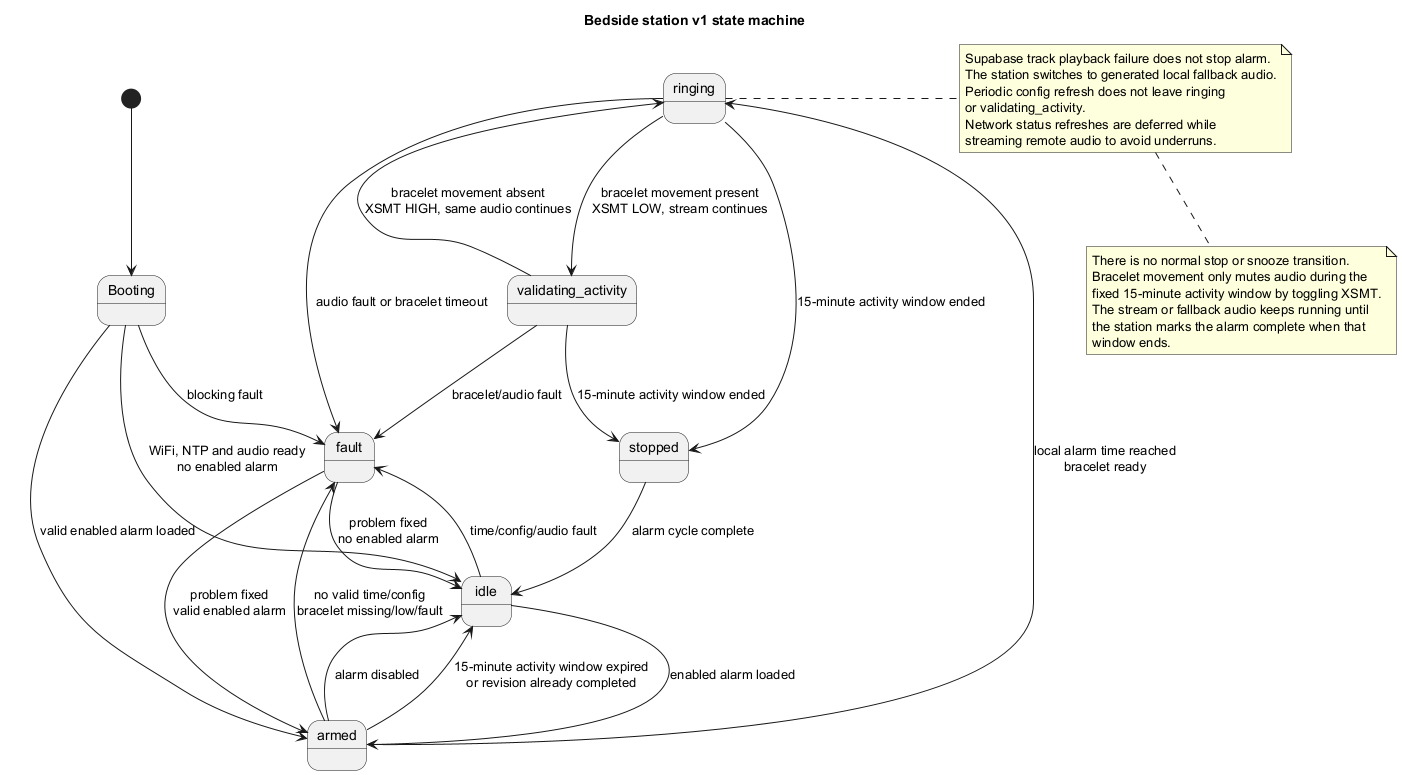
\includegraphics[width=\linewidth,height=0.72\textheight,keepaspectratio]{station_state_machine.png}
  \textbf{Diagramme: machine d'état v1 de la station}
\end{center}

Les états exposés par la station sont \texttt{idle}, \texttt{armed}, \texttt{ringing}, \texttt{validating\_activity}, \texttt{stopped} et \texttt{fault}. Le passage en \texttt{ringing} se produit lorsque l'heure locale configurée est atteinte et que les prérequis sont valides. Le passage en \texttt{validating\_activity} signifie que le bracelet signale du mouvement; la station coupe alors la sortie audio via \texttt{XSMT}, mais le cycle d'alarme continue.

La fenêtre d'activité dure quinze minutes à partir de l'heure configurée. À la fin de cette fenêtre, la station arrête le son et marque la révision comme terminée. Il n'y a pas de transition stop ou snooze normale depuis \texttt{ringing} ou \texttt{validating\_activity}.

\subsection{Défauts et fallback}

Avant l'alarme, les défauts bloquants incluent l'absence d'heure valide, l'absence de configuration valide, un bracelet manquant ou en défaut, une batterie bracelet trop basse et un problème audio. Dans ces cas, la station doit publier un défaut visible.

L'échec du streaming musical au moment du réveil n'est pas bloquant pour le réveil lui-même. La station bascule sur un son local généré, indépendant du réseau.

\section{Bracelet}

Le bracelet est un firmware PlatformIO Arduino pour ESP32-C3. Il lit le BMI270, calcule un score d'activité et envoie des paquets ESP-NOW à la station.

\begin{center}
  \centering
  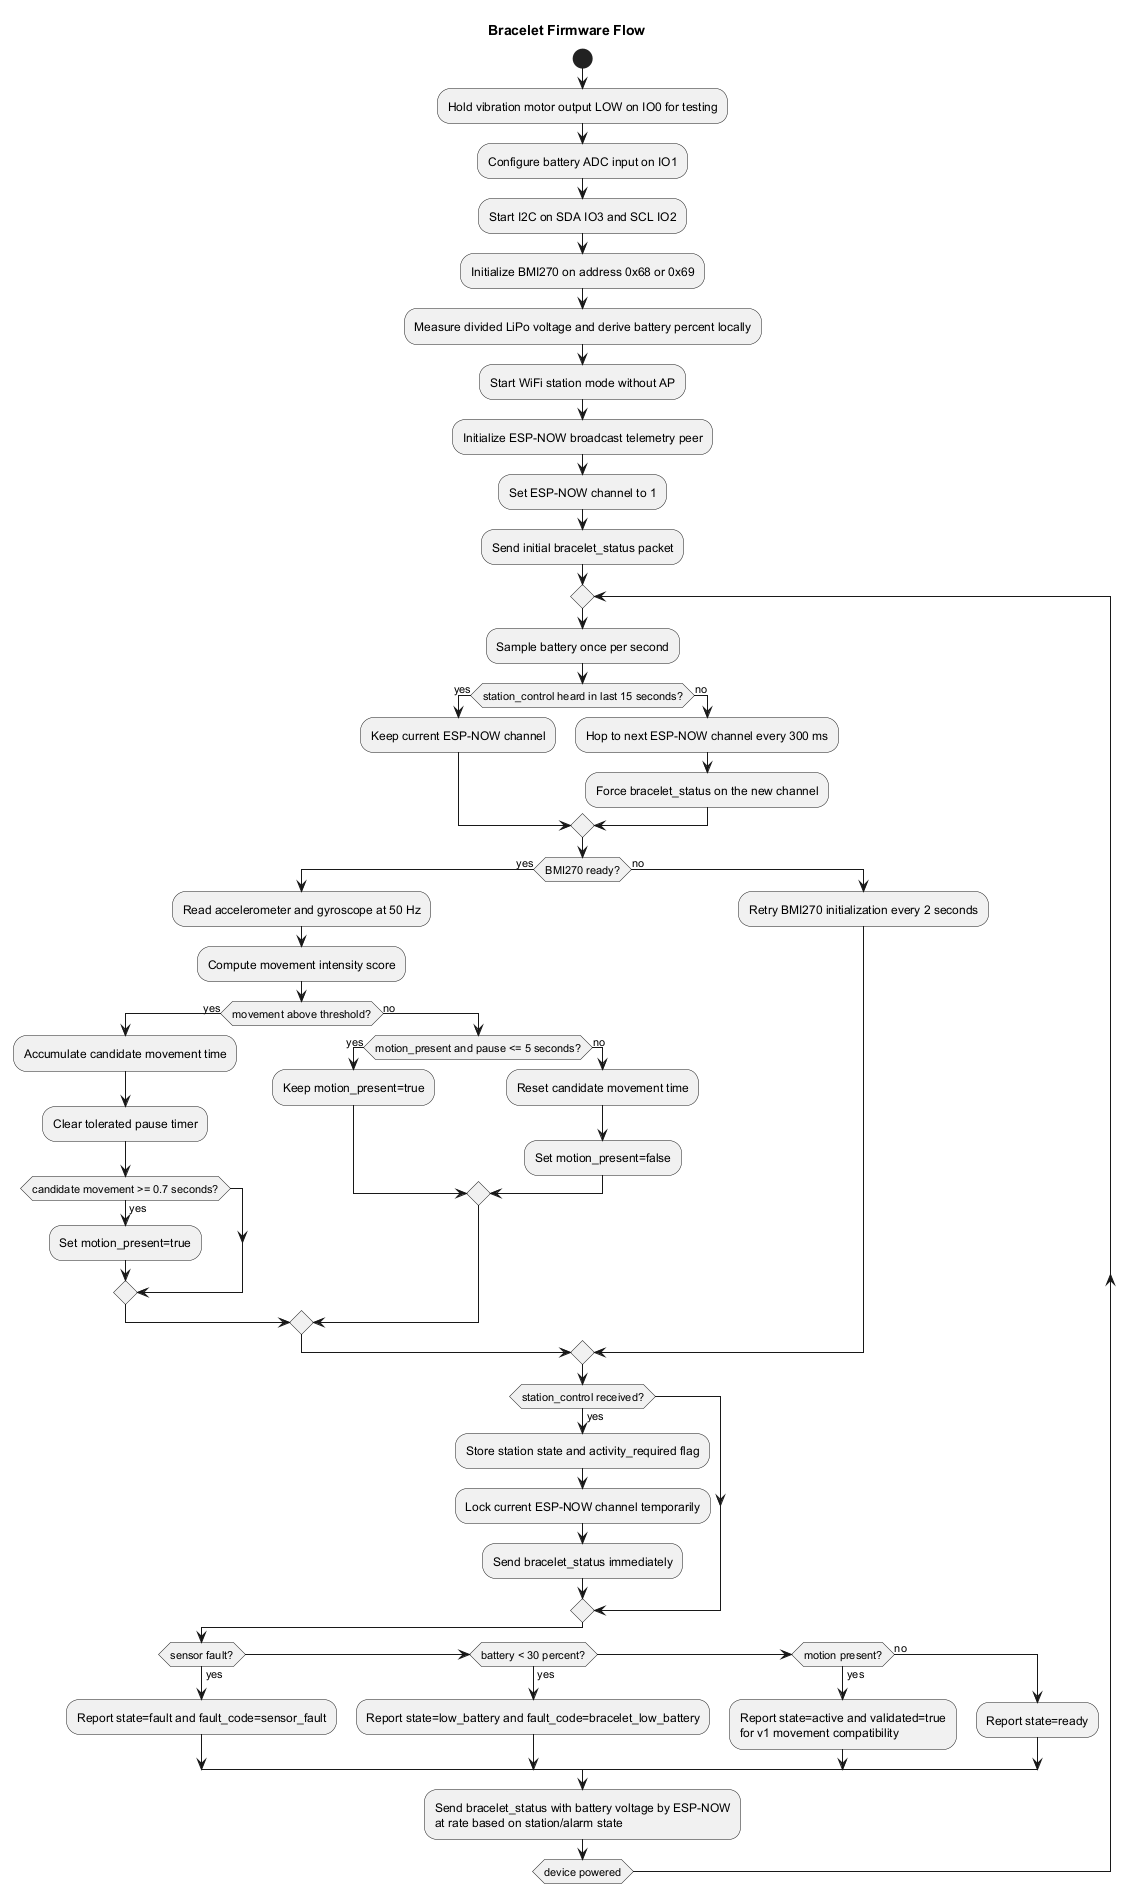
\includegraphics[width=\linewidth,height=0.72\textheight,keepaspectratio]{bracelet_firmware_flow.png}
  \textbf{Diagramme: flux firmware du bracelet}
\end{center}

\subsection{Activité}

Le firmware lit l'accéléromètre et le gyroscope à intervalle régulier. Il calcule un score d'activité sur 100 et maintient un booléen \texttt{motion\_present}. En v1, \texttt{validated=true} reflète le mouvement courant pour simplifier le contrat avec la station.

La logique actuelle confirme le mouvement après une courte durée continue et tolère une pause limitée afin d'éviter de couper immédiatement l'état actif sur une micro-interruption. Les seuils exacts devront rester ajustables après tests physiques.

\subsection{Flux ESP-NOW}

\begin{center}
  \centering
  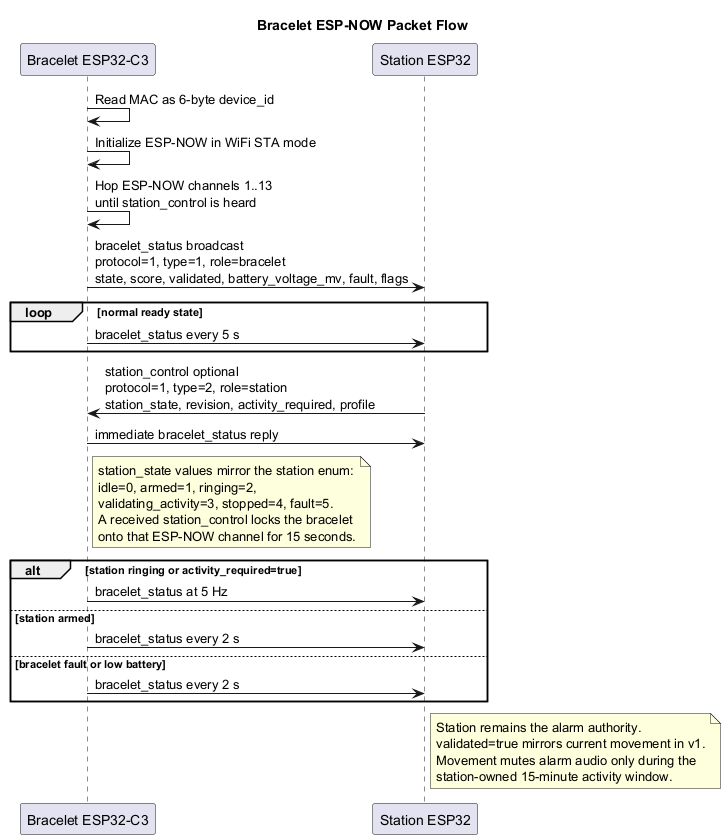
\includegraphics[width=\linewidth,height=0.72\textheight,keepaspectratio]{esp_now_packet_flow.png}
  \textbf{Diagramme: flux des paquets ESP-NOW}
\end{center}

Les paquets commencent par une version de protocole, un type de message, un rôle émetteur, un identifiant de périphérique, une séquence et un uptime. Le bracelet diffuse \texttt{bracelet\_status}. La station peut diffuser \texttt{station\_control}; le bracelet peut alors se verrouiller temporairement sur le canal reçu.

Le bracelet ne contacte pas Supabase. Il ne décide pas de l'état final de l'alarme.

\section{Contrats inter-systèmes}

\subsection{États}

Les états station et bracelet sont partagés entre firmware, Supabase et PWA. Ils doivent rester synchronisés avec \texttt{ARCHITECTURE.md}, le SQL Supabase et les types TypeScript.

\begin{itemize}
  \item Station: \texttt{idle}, \texttt{armed}, \texttt{ringing}, \texttt{validating\_activity}, \texttt{stopped}, \texttt{fault}.
  \item Bracelet: \texttt{unknown}, \texttt{charging}, \texttt{ready}, \texttt{active}, \texttt{validated}, \texttt{low\_battery}, \texttt{fault}.
\end{itemize}

\subsection{Codes de problème}

Les principaux codes v1 sont:

\begin{itemize}
  \item \texttt{none}, \texttt{wifi\_unavailable}, \texttt{supabase\_unavailable}, \texttt{time\_unknown};
  \item \texttt{no\_valid\_alarm\_config}, \texttt{music\_stream\_failed}, \texttt{fallback\_audio\_failed};
  \item \texttt{bracelet\_missing}, \texttt{bracelet\_low\_battery}, \texttt{bracelet\_fault};
  \item \texttt{sensor\_fault}, \texttt{audio\_fault}, \texttt{unknown\_fault}.
\end{itemize}

\subsection{Batterie}

La station et le bracelet publient des tensions batterie brutes. L'affichage en pourcentage est dérivé côté PWA. Pour v1, le bracelet est considéré faible sous 30\% et bloquant avant alarme sous 20\%. Si la tension ne peut pas être mesurée, le système doit publier une valeur inconnue plutôt que simuler une précision.

\section{Matériel}

Les composants listés dans \texttt{composants.txt} sont considérés comme fixes sauf validation explicite. Les éléments principaux sont:

\begin{itemize}
  \item ESP32 pour la station;
  \item ESP32-C3 pour le bracelet;
  \item BMI270 pour le mouvement;
  \item PCM5102A comme DAC I2S;
  \item PAM8403 comme amplificateur;
  \item batteries LiPo 1S;
  \item modules de charge IP2312;
  \item pogo pins, PTC réarmables et LDO 3.3 V.
\end{itemize}

Les changements de batterie, charge, connecteur, PCB, boîtier ou chaîne audio doivent être traités comme des décisions matérielles importantes.

\section{Structure du dépôt}

\begin{longtable}{>{\ttfamily}p{0.34\linewidth}p{0.58\linewidth}}
\toprule
\normalfont Chemin & Rôle \\
\midrule
\endhead
ARCHITECTURE.md & Contrats canoniques entre PWA, station, bracelet et Supabase. \\
database/supabase & SQL concret pour le backend v1. \\
code/app mobile & PWA Vue/Vite. \\
code/app mobile/UML & Diagrammes de cas d'utilisation et flux utilisateur. \\
code/boite hp & Firmware PlatformIO de la station. \\
code/boite hp/UML & Diagrammes d'architecture et d'état station. \\
code/bracelet & Firmware PlatformIO du bracelet. \\
code/bracelet/UML & Diagrammes firmware et ESP-NOW du bracelet. \\
schema/bracelet & Sources KiCad du bracelet. \\
doc & Rapport LaTeX et PDF généré manuellement. \\
\bottomrule
\end{longtable}

\section{Limites connues}

\begin{itemize}
  \item Le modèle Supabase sans authentification est uniquement un raccourci prototype personnel.
  \item La portée ESP-NOW doit être validée en conditions réelles.
  \item Les seuils d'activité et de batterie doivent être calibrés avec le matériel final.
  \item Le fallback local protège contre l'échec du streaming, mais ne remplace pas la configuration Supabase normale.
  \item Le rapport est un artefact manuel: il doit être mis à jour quand l'architecture, les contrats ou les comportements significatifs changent.
\end{itemize}

\section{Conclusion}

Le système Starter est organisé autour d'une séparation stricte des responsabilités. La PWA configure, Supabase stocke et expose, le bracelet mesure, et la station décide. Cette séparation permet de développer chaque partie indépendamment tant que les contrats de \texttt{ARCHITECTURE.md} restent respectés.

\end{document}
